\documentclass[tikz, border=20pt]{standalone}
\usepackage[utf8]{inputenc}
\usepackage{tikz}
\usetikzlibrary{positioning, fit, calc, shapes.geometric, arrows.meta, shadows.blur, backgrounds}
\usepackage{fontawesome5} 
\usepackage{helvet}
\renewcommand{\familydefault}{\sfdefault}

% --- Paleta de Colores ---
\definecolor{userPurple}{RGB}{147, 112, 219} 
\definecolor{itemBlue}{RGB}{70, 130, 180}    
\definecolor{itemRed}{RGB}{205, 92, 92}      
\definecolor{itemGreen}{RGB}{60, 179, 113}   
\definecolor{itemOrange}{RGB}{255, 165, 0}   
\definecolor{fusionGray}{RGB}{119, 136, 153} 
\definecolor{loraGold}{RGB}{218, 165, 32}    
\definecolor{bgGray}{RGB}{250, 250, 250}     

\begin{document}

\begin{tikzpicture}[
    node distance=1.2cm and 1.5cm,
    font=\sffamily\small,
    % Estilos
    block/.style={
        rectangle, 
        draw=black!60, 
        fill=white, 
        thick, 
        rounded corners=4pt, 
        minimum height=1.2cm, 
        text width=3.8cm, 
        align=center,
        blur shadow={shadow blur steps=3, shadow opacity=20}
    },
    input_node/.style={
        rectangle,
        rounded corners=6pt,
        draw=black!40,
        fill=white,
        thick,
        minimum height=0.9cm,
        text width=3.0cm,
        align=center,
        font=\sffamily\footnotesize
    },
    fusion/.style={
        block,
        fill=fusionGray!15,
        draw=fusionGray!80!black,
        minimum height=1cm,
        font=\sffamily\bfseries\small
    },
    operator/.style={
        circle, 
        draw, 
        thick, 
        fill=white, 
        inner sep=0pt, 
        minimum size=0.8cm,
        font=\large\bfseries
    },
    arrow/.style={
        -{Stealth[length=3mm, width=2mm]}, 
        thick, 
        draw=black!70,
        rounded corners=5pt
    }
]

    % =========================================================
    % 1. TOP SECTION (SALIDA)
    % =========================================================
    
    % AJUSTE 1: Etiqueta "Dot Product" movida ABAJO (below)
    % Esto libera completamente el espacio de arriba para la flecha de salida
    \node[operator, label={below:\textbf{Dot Product}}] (dot_prod) at (5.5, 13.5) {$\otimes$};
    
    \node[block, above=0.8cm of dot_prod, text width=3.5cm, fill=black!5, dashed] (output_prob) {
        \textbf{Similarity Score}\\
        \scriptsize Sigmoid($u^T v$)
    };
    \draw[arrow] (dot_prod) -- (output_prob);

    % =========================================================
    % 2. USER TOWER (Izquierda)
    % =========================================================
    
    \node[fusion] (user_fusion) at (0, 9.5) {
        User Fusion Layer\\
        \scriptsize Linear $\rightarrow$ LN $\rightarrow$ ReLU
    };

    \node[operator, below=0.8cm of user_fusion, label={135:\scriptsize Concat}] (user_concat) {$\parallel$};

    % --- Transformer ---
    \node[block, below=1.5cm of user_concat, xshift=-1.5cm, fill=userPurple!10, draw=userPurple!80!black] (transformer) {
        \textbf{Transformer Encoder}\\
        \scriptsize (SASRec Core)\\
        \scriptsize $L=2, H=4$
    };
    
    \node[block, below=0.6cm of transformer, fill=userPurple!05, draw=userPurple!50, minimum height=0.8cm] (pos_emb) {
        \scriptsize Positional Emb. $\oplus$ Item Emb.
    };
    
    \node[input_node, below=0.8cm of pos_emb] (in_hist) {
        \faHistory \ \textbf{History IDs}
    };

    % --- Demographics ---
    \node[block, right=0.8cm of transformer, fill=itemOrange!10, draw=itemOrange!80!black, text width=2.8cm] (demo_emb) {
        \textbf{Demographics}\\
        \scriptsize Gender + Country\\
        \scriptsize (Embeddings)
    };
    
    \node[input_node] (in_demo) at (demo_emb |- in_hist) {
        \faUser \ \textbf{User Profile}
    };

    % Conexiones User Tower
    \draw[arrow] (in_hist) -- (pos_emb);
    \draw[arrow] (pos_emb) -- (transformer);
    \draw[arrow] (in_demo) -- (demo_emb);
    
    \draw[arrow] (transformer.north) |- (user_concat);
    \draw[arrow] (demo_emb.north) |- (user_concat);
    \draw[arrow] (user_concat) -- (user_fusion);

    % =========================================================
    % 3. ITEM TOWER (Derecha)
    % =========================================================
    
    \node[fusion] (item_fusion) at (11, 9.5) {
        Item Fusion Layer\\
        \scriptsize Linear $\rightarrow$ BN $\rightarrow$ Drop
    };

    \node[operator, below=0.8cm of item_fusion, label={180:\scriptsize Concat}] (item_concat) {$\parallel$};

    % --- Stack de Encoders ---
    \node[block, below=1.5cm of item_concat, fill=itemGreen!10, draw=itemGreen!80!black] (text_enc) {
        \textbf{Text Encoder}\\
        \scriptsize mDeBERTa-v3
    };
    \node[draw=loraGold, fill=loraGold!20, rounded corners=2pt, inner sep=3pt, font=\tiny\bfseries, anchor=north east, yshift=2pt] at (text_enc.north east) {LoRA};

    \node[block, below=0.6cm of text_enc, fill=itemRed!10, draw=itemRed!80!black] (visual_enc) {
        \textbf{Visual Encoder}\\
        \scriptsize ResNet18 (ImageNet)
    };

    \node[block, below=0.6cm of visual_enc, fill=itemBlue!10, draw=itemBlue!80!black] (audio_enc) {
        \textbf{Audio Encoder}\\
        \scriptsize ResNet18 (Spectrogram)
    };
    
    \node[block, below=0.6cm of audio_enc, fill=itemOrange!10, draw=itemOrange!80!black] (tab_enc) {
        \textbf{Tabular Encoder}\\
        \scriptsize MLP (Features)
    };

    % --- Input Unificado ---
    \node[input_node, below=1.2cm of tab_enc, text width=5.5cm] (in_item_data) {
        \faBoxOpen \ \textbf{Item Raw Data}\\
        \scriptsize (Lyrics, Cover, Audio, Metadata)
    };

    % --- Conexiones Entrada ---
    \draw[arrow] (in_item_data.north) -- (tab_enc.south);
    \draw[arrow] (in_item_data.west) -- ++(-0.5, 0) |- (audio_enc.west);
    \draw[arrow] (in_item_data.west) -- ++(-0.5, 0) |- (visual_enc.west);
    \draw[arrow] (in_item_data.west) -- ++(-0.5, 0) |- (text_enc.west);
    
    % --- Conexiones Salida (Bus Derecho) ---
    \draw[arrow] (text_enc.east) -- ++(0.4, 0) |- (item_concat);
    \draw[arrow] (visual_enc.east) -- ++(0.8, 0) |- (item_concat);
    \draw[arrow] (audio_enc.east) -- ++(1.2, 0) |- (item_concat);
    \draw[arrow] (tab_enc.east) -- ++(1.6, 0) |- (item_concat);
    
    \draw[arrow] (item_concat) -- (item_fusion);

    % =========================================================
    % 4. CONEXIONES FINALES PERFECTAS
    % =========================================================
    
    % AJUSTE 2: Usamos '|-' (Vertical-Horizontal) automático.
    % 'pos=0.75' pone la etiqueta en el tramo horizontal final.
    % 'above=3pt' asegura que no toque la línea.
    
    % User Side (Left)
    \draw[arrow] (user_fusion.north) |- (dot_prod.west) node[pos=0.75, above=3pt, font=\bfseries] {$u$};
    
    % Item Side (Right)
    \draw[arrow] (item_fusion.north) |- (dot_prod.east) node[pos=0.75, above=3pt, font=\bfseries] {$v$};

    % =========================================================
    % 5. BACKGROUNDS
    % =========================================================
    
    \begin{scope}[on background layer]
        \node[fit=(user_fusion)(in_hist)(in_demo)(demo_emb)(transformer), fill=bgGray, rounded corners=20pt, draw=black!10, inner sep=35pt, label={[anchor=north west, inner sep=15pt, font=\bfseries\color{gray!80}]north west:User Tower}] (user_bg) {};
        
        \coordinate (aux_right) at ($(text_enc.east)+(1.8,0)$); 
        \coordinate (aux_left) at ($(text_enc.west)+(-1.2,0)$); 
        
        \node[fit=(item_fusion)(tab_enc)(in_item_data)(aux_right)(aux_left), fill=bgGray, rounded corners=20pt, draw=black!10, inner sep=35pt, label={[anchor=north east, inner sep=15pt, font=\bfseries\color{gray!80}]north east:Item Tower}] (item_bg) {};
    \end{scope}

\end{tikzpicture}
\end{document}